 %=================================================================
\documentclass[Unknown,article,submit,moreauthors,pdftex,10pt,a4paper]{Definitions/mdpi} 
\usepackage{siunitx}
\usepackage{multirow}
\preto{\abstractkeywords}{\nolinenumbers}
\firstpage{1} 
\makeatletter 
\setcounter{page}{\@firstpage} 
\makeatother
\pubvolume{xx}
\issuenum{1}
\articlenumber{5}
\pubyear{2018}
\copyrightyear{2018} 
%\externaleditor{Academic Editor: name}
\history{Received: date; Accepted: date; Published: date}
 
% Full title of the paper (Capitalized)
% \Title{Effect of Nanovoid on Fracture Process of Two-Phase $\gamma$($\rm TiAl$)+$\alpha_2$($\rm Ti_3Al$) Alloy}
\Title{Micromechanism of  Cold Deformation of Two Phase Polycrystalline Ti-Al Alloy with void}
% Author Orchid ID: enter ID or remove command
\newcommand{\orcidauthorA}{0000-0001-8385-4439} % Add \orcidA{} behind the author's name
\newcommand{\orcidauthorB}{0000-0002-9582-6301} % Add \orcidB{} behind the author's name

% Authors, for the paper (add full first names)
\Author{Author \orcidA{}}
%\Author{Ruicheng Feng $^{1,2}$\orcidA{}, Maomao Wang $^{1}$\orcidB{}}

% Authors, for metadata in PDF
%\AuthorNames{Maomao Wang $^{1,\dagger,\ddagger}$\orcidB{}, Firstname Lastname and Firstname Lastname}

% Affiliations / Addresses (Add [1] after \address if there is only one affiliation.)
\address{%
% $^{1}$ \quad School of Mechanical and Electronical Engineering, Lanzhou University of Technology, Lanzhou 730050, China; frcly@163.com (R.F.); 15620864891@163.com (M.W.)\\
$^{1}$ \quad School of Mechanical and Electronical Engineering, Lanzhou University of Technology, Lanzhou 730050, China;\\
% $^{2}$ \quad Key Laboratory of Digital Manufacturing Technology and Application, Ministry of Education, Lanzhou University of Technology, Lanzhou 730050, China
%*; e-mail@e-mail.com}
$^{2}$ \quad State Key Laboratory of Advanced Processing and Recycling of Non-ferrous Metals, Lanzhou University of Technology, Lanzhou 730050, China}
% Contact information of the corresponding author
\corres{Correspondence: e-mail@e-mail.com; Tel.: +x-xxx-xxx-xxxx}

% Current address and/or shared authorship
%\firstnote{Current address: Affiliation 3} 
%\secondnote{These authors contributed equally to this work.}
% The commands \thirdnote{} till \eighthnote{} are available for further notes

%\simplesumm{} % Simple summary

%\conference{} % An extended version of a conference paper

% Abstract (Do not insert blank lines, i.e. \\) 
\abstract{Cold deformation behavior of poly crystalline metallic material is affected by intrinsic defects such as dislocation, void, inclusion etc.  Existing studies on $\alpha_2(\rm{Ti_3Al})$+$\gamma(\rm{TiAl})$  two phase Ti-Al alloy cover about deformation behavior mainly on macro scale. This paper focuses on the cold deformation mechanism of two phase Ti-Al alloy at micro scale, and the role of void in deformation process. Molecular dynamics simulations were performed to study the evolution of micro structure of material under uniaxial tension. Interaction between spherical nano void with different size and position was also examined in the simulation. The results show that (1) $\gamma$ phase is the major deformation source of the two phase alloy; (2) void detracts the strength of the two phase alloy, while the position of void affect the degree of this subtraction, voids located at the boundary of $\alpha_2$/$\gamma$ phase have significant detraction to strength.}
% Keywords
\keyword{two phase Ti-Al alloy, void, molecular dynamics, cold deformation}

%%%%%%%%%%%%%%%%%%%%%%%%%%%%%%%%%%%%%%%%%%
\begin{document}

\section{Introduction}
% and brittle rapture failure 
Titanium aluminum based intermetallic alloys are promising high temperature structural materials because of their great corrosion resistance and strength at high temperature. Compared with nickle based alloy, Ti-Al based alloys have lower density and are pron to be utilized in combustion engine, turbine, and other components working at high temperature from 500 \si{\degreeCelsius} to 900 \si{\degreeCelsius} \cite{Clemens2016}. The performance of inner combustion engine with components made of Ti-6Al-4V was improved 20\% because the weight of components decreased from 30\% to 40\% \cite{Bewlay2016}. With the advancement of non-ferrous metallurgy, Ti-Al based alloy components have better economic efficiency than ever before. Ti-Al based alloys have good prospects for applications in aerospace and automobile industry. 
Poor ductility of Ti-Al alloy at room temperature strongly affects the safety of structures like turbo of aircraft engine and combustion generator \cite{Munz2017}. Deformation phenomena of Ti-Al alloys have been widely studied in order to overcome the problems associated with the limited ductility and damage tolerance.  Much of the work has been performed on single phase $\gamma$-TiAl alloys and polysynthetically twinned crystals (PTC)\cite{Appel2016}. Rapture failure at the macroscopic scale can be attributed to abrupt nucleation, growth and propagation of cracks, but at the microscopic scale defects are initially formed in the casting process, such as voids and inclusions \cite{Tang2014}. Numerous studies cover a wide range of factors such as alloy composition, microstructure and deformation temperature, some reports come up with the idea that two phase titanium aluminum alloys with proper phase distribution and grain size exhibit better mechanical performance compared with monolithic constituents $\gamma$(TiAl) and $\alpha_2$($\rm Ti_3Al$) alloy \cite{Kim1995}. 
void can be produced due to specific volume differences induced by precipitation, different thermal expansion or shrinkage upon heating or cooling the specimen. It has been known that nucleation, growth and coalescence of voids are deemed as the primary mechanism of ductile material fracture, in which void growth is particularly important \cite{Hempel2017a}. The initiation of crack at microscopic scale is a dynamic process, which results in difficulties on study of mechanisms about deformation and cracking, these defects are known playing a fundamental role in the deformation of materials. Multiscale method has been applied to study deformation behavior of polycrystal with single aluminum \cite{Groh2009} and titanium element respectively \cite{Liu2018}. It's necessary to carefully examine the revolution of defects and its influence on the fracture process at atomic scale. The effect of void is another great concern about properties and deformation mechanism of TiAl alloy.  Therefore, it is necessary to study the deformation response of intermetallics structural materials with the consideration of microstructure evolution. Previous study on void growth in single crystal $\gamma$-TiAl reveals that void with high volume fraction detracts yield strength \cite{Tang2014, Xu2011}. Evolution of void in ductile polycrystalline was studied in nanoscale with molecular dynamics(MD) simulations, \cite{Jing2018a,Elkhateeb2018}, voids inside material are sources of dislocation and affects the properties of materials differently because of differences in size and position.  The deformation and fracture mechanisms in the duplex microstructure are plasticity induced grain boundary decohesion and cleavage, while those in the lamellar micro-structure are interface delamination and cracking across the lamellar \cite{Tang2014}. It reveals that existence of voids alone may contribute to strain hardening because they are barriers to dislocation movement in ductile fcc structure metal\cite{Xiong2015}. However, few literature covers about deformation mechanism of two phase Ti-Al alloy and the role of void in atomic scale. Defects are inevitable as micro-pores and loosen from casting, and in the actual work environment with radiation. A lot of work carried out on the effect of various defects on the behavior of different materials, showing that point defects may affect the properties of materials greatly. The mechanical performance of irradiated copper is affected by the interaction between irradiation and dislocation \cite{Kiener2011}. Vacancy concentration in single crystal and polycrystal Fe–40 at. Al bulk results in an increase of strength \cite{Yang1998}. Ti-Al alloy is a type of typical brittle material, thus it can be assumed that its properties are sensitive to the existence of void. Surface defects such as small notches can cause low and high cycle fatigue strength of the Ti–47Al–2W–0.5Si alloy \cite{Nazmy2001}, and the strength of single crystal $\gamma$-TiAl is also lowered by point defect \cite{Wu2016}. The resistance of Ti–6Al–4V alloy, which was processed for typical fan blade applications, to high-cycle fatigue in the presence of foreign- object damage was reduced due to earlier crack initiation.  The nucleation and subsequent near-threshold growth of crack was primarily affected by the stress concentration associated with the foreign-object damage and the presence of small cracks in the damaged zone. Due to difficulties in observing the dynamic process during deformation wit experiments, MD simulation has become an effective method to investigate micro deformation mechanism. Defects such as grain boundary, void and segregation play significant roles in the process of fracture \cite{Larsen2016}. This paper focus on the evolution of microstructure, tending to find out its connection to cold deformation behavior of two phase TiAl alloy. MD simulation including model creation and analysis method is given in Section \ref{section:method}, Results and discussion are in Section \ref{section:RD}.

\section{Molecular Dynamics Simulation }\label{section:method}
\subsection{Atomic Potential}

The interaction of particle in the material is determined by interatomic potential. Many reported simulation cases of deform and crack propagation in metal materials were performed with embedded atomic method due to its better accuracy in metal lattice compare with F-S and L/J \cite{Ko2015,Zepeda-Ruiz2017,Fan2018a}. Embedded atom method (MEAM) potential developed by Zope and Mishin \cite{Zope2003} was used in the study. The simulation is submitted by MD simulations with the Large-scale Atomic/Molecular Massively Parallel Simulator (LAMMPS) open-source code \cite{Plimpton1995}. We performed constant-pressure and constant-temperature (NPT) molecular dynamics simulation at room temperature (298K). The definition of potential is as following:
	
\begin{equation} \label{eq:eam} 
E_{total}= \displaystyle\sum F_i(\rho_{h,i})+\frac{1}{2}\sum_i\sum_{j(\neq1)}\phi_{ij}(R_{ij})
\end{equation}
where $E_{total}$ is the total energy of the system, $\rho_{h,i}$, is the host electron density at atom $i$ due to the remaining atoms of the system, $F_i(\rho)$ represents the energy for embedding atom $i$ into the background electron density $\rho$, and $\phi_{ij}(R_{ij})$ gives the core-core pair repulsion between atoms $i$ and $j$ separated by the distance $R_{ij}$. It can be noted that $F_i$ only depends on the element of atom $i$ and $\phi_{ij}$ only depends on the elements of atoms $i$ and $j$. 

\subsection{Model Creation of Crystalline}
\begin{figure}[ht]
	\centering
	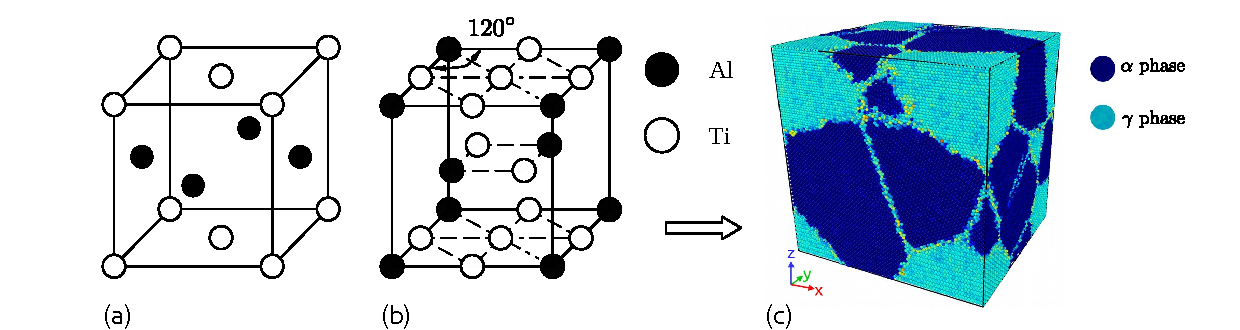
\includegraphics[width=1\linewidth]{img/modeling}
	\caption{Unit cell of \rm{TiAl} (a), $\rm{Ti_3Al}$ (b) and two phase Ti-Al model (c)}
	\label{fig:tial-cell}
\end{figure}

\begin{table}[ht]
	\caption{Parameters of nanocrystalline}
	\centering
	\begin{tabular}{c c c l}
	\toprule
	\textbf{Phase}			& {Space group}		& {Designation} 		& {Parameters} \\
	\midrule
	$\alpha_2$ - $\rm{Ti_3Al}$		& $\rm P6_3/mmc$ 	& $\rm 0_{19}$ 		& $a$ = 0.5765 \\
		&					&					& $c$ = 0.46833 \\
	$\gamma$ - $\rm{TiAl}$ 		& $\rm tP4$ 		& $\rm L1_0$		& $a$ = 0.3997 \\
		&					&					& $c$ = 0.4062 \\			
	\bottomrule
	\end{tabular} 
	\label{tab:lattice_parameter}
\end{table} 

Two phase Ti-Al alloy is composed of $\gamma $-TiAl and $\alpha_2$-$\rm Ti_3Al$ has a fcc type cell with an $L1_0$ structure, and $\alpha_2$-$\rm Ti_3Al$ has a hcp structure, these two types of initial cells are shown in Fig. \ref{fig:tial-cell}, constructing parameters of the two type of unit cell are given by table \ref{tab:lattice_parameter}. Periodic boundary conditions (PBC) are applied along three directions, which makes polycrystal with periodic nanovoid structures. The initial dimension of simulation cell is $L_x =200$ \si{\angstrom}, $L_y = $180\si{\angstrom}, $L_z = 210$ \si{\angstrom}, and each model contains about 460,000 atoms. The grain orientation and size were randomly created with Voronoi method by code ATOMSK \cite{Hirel2015}, and resulting in the arbitrary shape and orientation of the grains. Uniaxial load was applied to the model at a strain rate of $5\times10^8\ \rm{s}^{-1}$. 
% In order to study the deformation mechanism of the two phase alloy and the effect of void, three types of models were created: Type-1.model without any void; Type-2. models with different size void inside $\alpha_2$ phase; Type-3. models with void at $\alpha_2-\gamma$ interface. \ref{tab:lattice_parameter}. The simulation cells of two phase polycrystalline with an initially spherical void at different position are shown in figure .
\subsection{Analysis method}
In order to identify typical defects in the deformed model, a hybrid analysis method was used with free code ovito\cite{Stukowski2010a}.Dislocation is visualized by DXA method, and Centro-symmetry parameter(CSP) is used to tell grain boundary from  $\alpha_2$ phase and $\gamma$ phase. The definition of CSP is as following:

	\begin{equation} \label{eq:csp} 
	P = \displaystyle\sum_{i=1}^{6}|\vec{R_i}+{\vec{R}}_{i+6}|^2
	\end{equation}
	
where $\vec{R_i}$ and ${\vec{R}}_{i+6}$ are the vectors corresponding to the six pairs of opposite nearest neighbors in the fcc lattice. The centro-symmetry parameter(CSP) is zero for atoms in a perfect lattice. In other words, if the lattice is distorted, the value of P will not be zero. Instead, the parameter will have a value within the range corresponding to a particular defect. By removing all the perfect and surface atoms within the bulk, atoms around defected zone are visualized. 
 
\section{Results and Discussion}\label{section:RD}

\begin{figure}[ht]
	\centering
	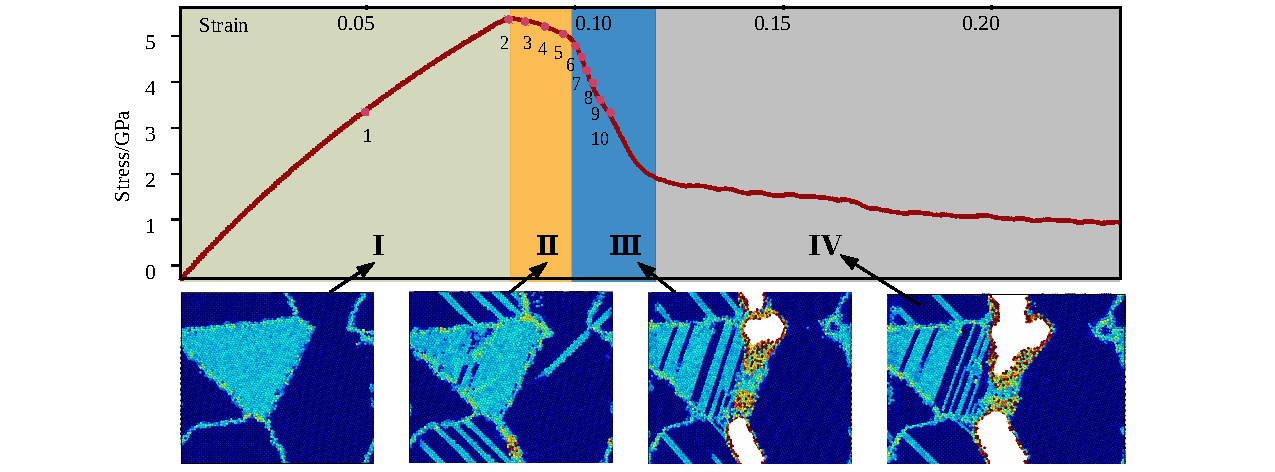
\includegraphics[width=1\linewidth]{img/tens}
	\caption{Deformation process of the model without void}
	\label{fig:deformation-pf}
\end{figure}


%	/home/alex/Documents/violet/draft/img/perfect-line.pdf
Deformation process of the model without void is shown in Fig. \ref{fig:deformation-pf}. The strength of the model without void is 5.3 GPa. According to stress response under constant rate of strain rate, the whole tensile process can be divided into four stages: 
stage - \uppercase\expandafter{\romannumeral1}: elastic stage, from $\epsilon = 0$ to $\epsilon = 0.092$, including key point 1,
stage - \uppercase\expandafter{\romannumeral2}: yield stage, ranging from $\epsilon = 0.092$ to $\epsilon = 0.101$, including key points 2 to 6,
stage - \uppercase\expandafter{\romannumeral3}: cracking stage, ranging from $\epsilon = 0.101$ to $\epsilon = 0.112$, including key point 7 to 10,
stage - \uppercase\expandafter{\romannumeral4}: fracture stage. Following discussion concentrates on deformation phenomena that rely on the elastro-plastic codeformation of the $\gamma$ and $\alpha_2$ phases and on the particular point defect situation occurring in two phase alloys. 

\begin{table}[ht]
	\caption{Key points during tensile process}
	\centering
	\begin{tabular}{l c c c c c c c c c c}
		\toprule
		\textbf{Number} &1 &2 &3 &4 &5 &6 &7 &8 &9 &10\\		 
		\midrule
		\textbf{Stage} &\uppercase\expandafter{\romannumeral1} &\uppercase\expandafter{\romannumeral1} &\uppercase\expandafter{\romannumeral2} &\uppercase\expandafter{\romannumeral2} &\uppercase\expandafter{\romannumeral2} &\uppercase\expandafter{\romannumeral2} &\uppercase\expandafter{\romannumeral3} &\uppercase\expandafter{\romannumeral3} &\uppercase\expandafter{\romannumeral3} &\uppercase\expandafter{\romannumeral3}	 \\
		\midrule
		% Time/ps	& 0 & 0.15 & 0.16 & 0.17 & 0.18 & 0.19 & 0.Fu = sin20 & 0.21 & 0.22 & 0.23 \\
		% \midule
		\textbf{Strain}	& 0.05 &  0.088 & 0.092 & 0.096 & 0.099 & 0.101 & 0.104 & 0.107 & 0.110 & 0.112  \\
		\bottomrule
	\end{tabular} 
	\label{tab:key-point}
\end{table}

 


% Due to this effect ( $\alpha_2$ + $\gamma$ ) alloys exhibit some remarkable properties that are unlike those of either constituent.
\subsection{Deformation Mechanism of Two Phase TiAl Alloy without voids}
Snapshots of atom configuration at the 3 of 10 key points are shown by Fig. \ref{fig:Defect}.  Atoms with ordered configuration  of $\gamma$ phase grains have been removed in Fig. \ref{fig:Defect}(a) and (b),\ $\alpha_2$ phase and defects inside grains have been left. Similarly, $\gamma$ phase grain have been removed in Fig. \ref{fig:Defect}(c) and (d), the defects of $\alpha_2$ phase have been left.  The results show that, at stage \uppercase\expandafter{\romannumeral1}, the structure of material is under typical elastic deformation, the size of simulation box enlarged due to the loading. In this stage, deformation of the two phase are compatible. Emission of dislocation and evolution of defects initiated at the end of stage \uppercase\expandafter{\romannumeral1}. A  great number of dislocation emitted inside $\gamma$ phase at earlier part of stage \uppercase\expandafter{\romannumeral2}, however, the dislocation inside $\alpha_2$ phase was emitted at the end of stage \uppercase\expandafter{\romannumeral2} is shown by Fig. \ref{fig:Defect}(c).  
\begin{figure}[ht] 
	\centering
	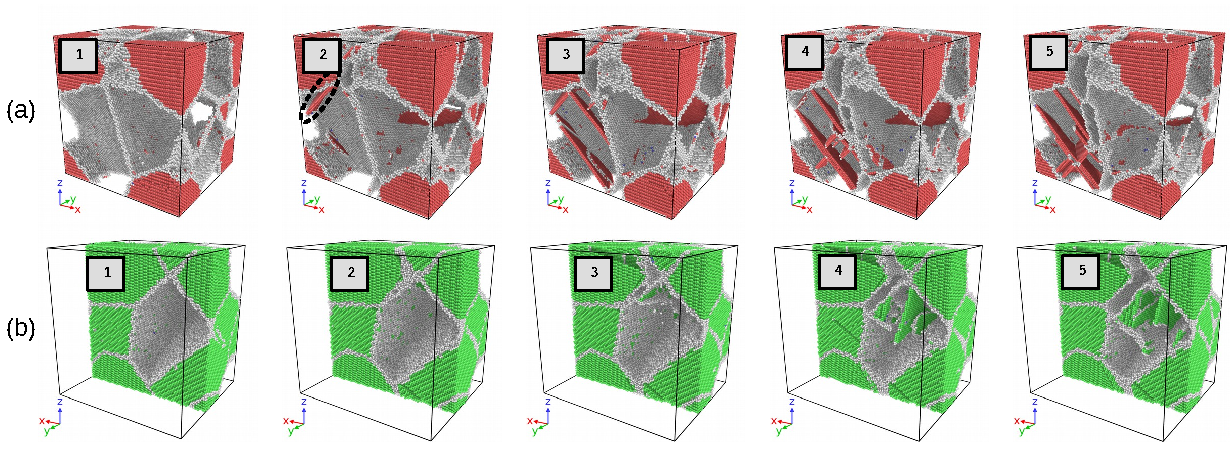
\includegraphics[width=1\linewidth]{img/def-box}
	\caption{Microstructure evolution inside $\gamma$ phase(a,b), $\alpha_2$ phase(c,d) during yield stage}
	\label{fig:Defect}
\end{figure}
Experiments have shown that the velocity of dislocation motion is sensitive to stress and temperature\cite{Stein1960}. The brittleness of two phase Ti-Al alloy attributed to the poor mobility of dislocation at room temperature. Velocity of a screw dislocation can be estimated by Escaig's elastic model \cite{Escaig1968}, it can be written as:
\begin{equation}\label{eq:temp-dis}
v = v_0\ e^{-\Delta H(\tau^*)/kT}
\end{equation}
where the prefactor $v_0$ gives the velocity that would be obtained for each potential mobility, $L$ represents the free length of screw character of dislocation, $\Delta H(\tau^*)$ is activation enthalpy determined by loading conditions. The effect of temperature on the mobility can be evaluated under different loading conditions, thus we chose  $\tau_1^*>\tau_2^*>\tau_3^*$ in formulation (\ref{eq:temp-dis}), normalized velocity of dislocation motion is shown by Fig. \ref{fig:temp}. The velocity  of dislocation movement rise along with increase of  stress, the mobility  of dislocation is relatively poor at 298 K. Due to motion of dislocations is inactive inside $\alpha_2$ phase,  typical strengthening mechanism closely related with interaction between grain boundary and dislocation is not dramatic at room temperature, piling up of dislocations is not observed in this simulation, which is shown in Fig. \ref{fig:Defect}.
\begin{figure}[ht]
	\centering
	\begin{minipage}{0.495\textwidth}
		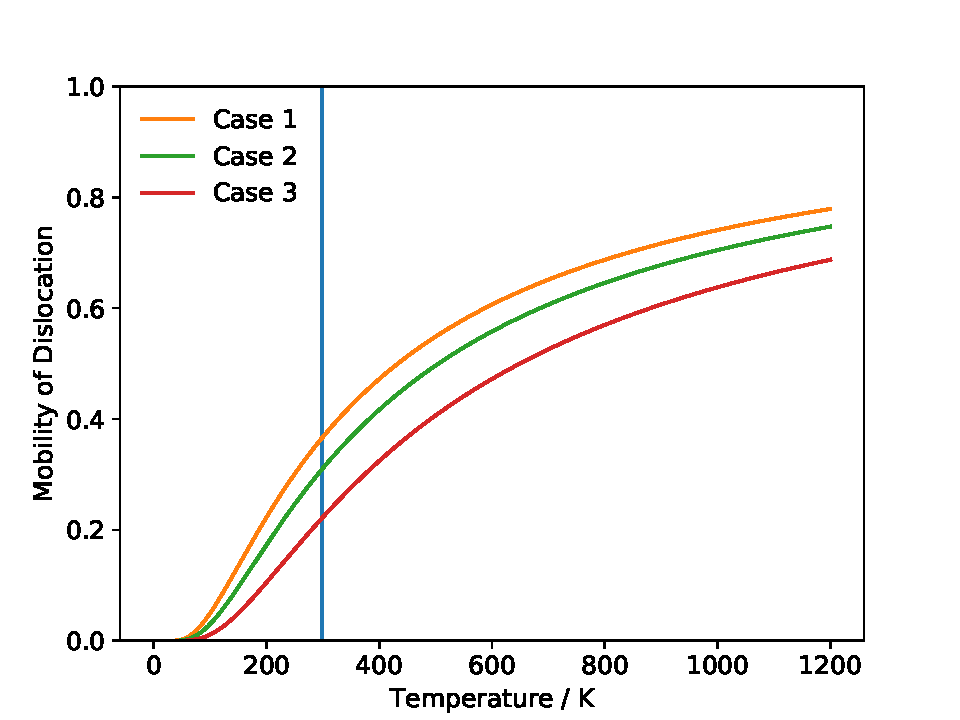
\includegraphics[width=1\linewidth]{img/temp}
		\centering
		\caption{Normalized velocity of dislocation motion under different loading conditions}
		\label{fig:temp}
	\end{minipage}	
	\hfill
	\begin{minipage}{0.495\textwidth}		
		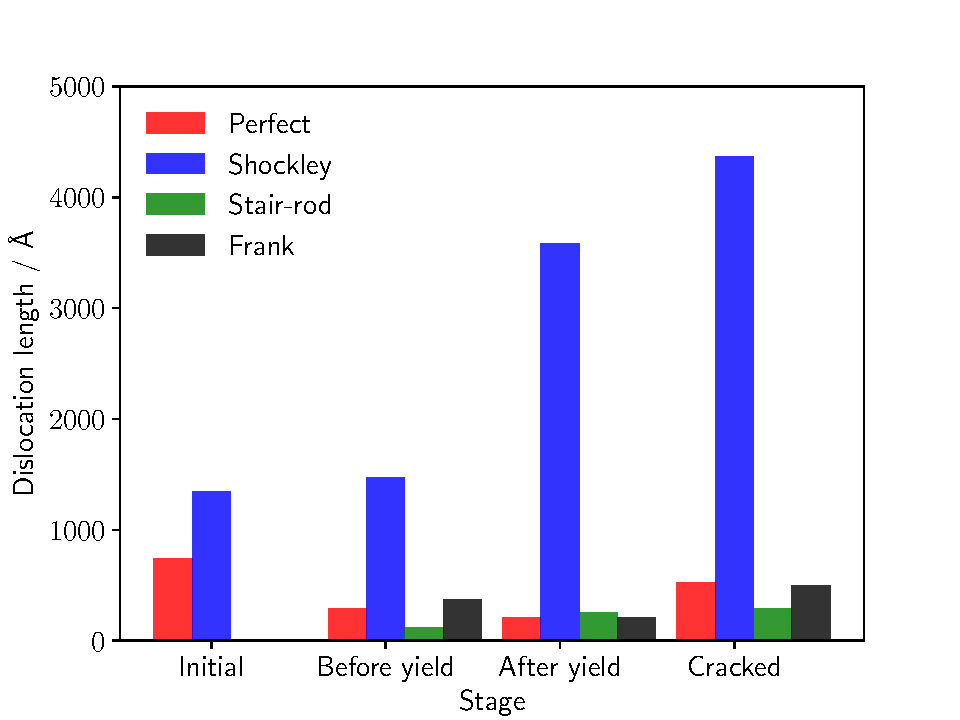
\includegraphics[width=1\linewidth]{img/dis-summary}
		\centering
		\caption{Dislocation length under differentstrain }
		\label{fig:disum}
	\end{minipage}
\end{figure}

Length of different types of dislocations are given at four stages in Fig. \ref{fig:disum}. Dislocations are recognized and identified using the dislocation analysis (DXA) of ovito. The length of Shorckley dislocation with Burgers vector $1/6[1 1 2]$ increased sharply during yield stage of the deformation process in Fig. \ref{fig:disum}, but the length of perfect dislocation fluctuated at a low level. Perfect  dislocations split into Shockley partial dislocations, this decomposition process  can be given by formulation (\ref{eq:dis-1}) and (\ref{eq:dis-2}). The structure spontaneously transformed into intrinsic stacking fault (ISF), which can be observed in Fig. \ref{fig:Defect}(a). 

%\begin{equation}\label{eq:dis-1}
%[\ 0\ 1\ \overline{1}\ ] \to 1/2 [\ 1\ 1\ \overline{2}\ ]+1/2[\ \overline{1}\ 1\ 0\ ]\\
%\end{equation}

\begin{equation}\label{eq:dis-1}
1/2 [\ 0\ 1\ 1\ ] \to 1/6[\ 1\ 1\ 2\ ]+1/6[\ \overline{1}\ 2\ 1\ ]
\end{equation}
\begin{equation}\label{eq:dis-2}
1/2 [\ 1\ 0\ \overline{1}\ ] \to 1/6 [\ 1\ 1\ \overline{2}\ ] + 1/6[\ 2\ \overline{1}\ \overline{1}\ ]
\end{equation}
Interaction between dislocations with Burgers vector of $1/6 [112] $ and $ 1/6 [11\overline{2}]$ follows the decomposition of perfect dislocation. The process produced leading dislocation and trailing dislocation, when the two leading Shockley partials combined, they form Lomer–Cottrell junction, a separate dislocation. It's sessile in the slip plane, playing a role of barrier against other dislocations in the plane. This process is given by
\begin{equation}\label{eq:dis-3}
1/6 [\ 1\ 1\ 2\ ] + 1/6 [\ 1\ 1\  \overline{2}\ ] \to 1/3 [\ 1\ 1\ 0\ ]
\end{equation}
According to the  results calculated by first principle, the stacking fault energy of TiAl is much smaller than $\rm{Ti_3Al}$, as a consequence, calculated shear strength of TiAl and $\rm{Ti_3Al}$is 4.1 Gpa and 2.86 Gpa along their easy slip plane respectively\cite{Liu2007}. This calculation reveals that tensile behaviour in single crystal is mainly controlled by the type of the structure. However, in two phase Ti-Al alloy, deformation of $\alpha_2$ phase is earlier than $\gamma$ phase during yield stage, thus local displacement of two phases are incompatible during yield stage.  Mobility of dislocation is affected by structure of crystal, loading condition and temperature. And $\alpha_2$ phase is made up of hcp structured grain, grains with this type of structure possess less slip system compared with grain with fcc structure \cite{Zhu2012}, thus $\alpha_2$ phase is difficult do deform under uniaxial tensile loading. 

Main reason for the unequal strain partitioning between the $\alpha_2$ and $\gamma$ phase is the strong plastic anisotropy of  $\alpha_2$ phase. TEM examinations performed on tensile tested lamellar alloys have revealed that the limited plasticity of $\alpha_2$ phase is carried by local slip of dislocations with the Burgers vector $1/3[11\overline{2}0]$ prism planes shown by Fig. \ref{fig:Defect}(b), which is by far the easiest slip system in $\alpha_2$ single crystals.  Dislocation neighboring interfaces often needs to be transformed. For example, an ordinary 1/2 [110] dislocation gliding in one $\gamma$ grain has to be converted into $[101]$ super dislocation when the double Burgers vectors gliding in an adjacent $\gamma$ grain. At the $\alpha_2/\gamma$ interface, dislocations existing in $D0_{19}$ structure  transform into dislocations, which is consistent with the $\rm{L1_0}$ structure. These core transformations are associated with the change of the dislocation line energy because of the differences of the length and the shear module.  Pyramidal slip of the $\alpha_2$ phase is required when slip is forced to cross $\alpha_2$ phase, this process needs an extremely high shear stress.


\subsection{The effect of void on the strength of material}

\begin{figure}[ht]
	\centering
	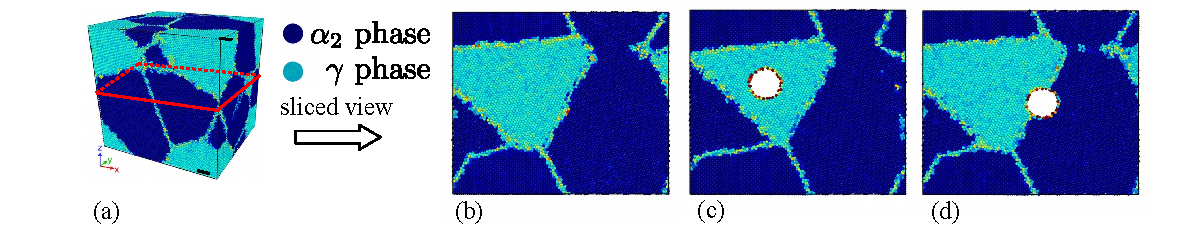
\includegraphics[width=1\linewidth]{img/slice-view}
	\caption{ Model with no void (b), with void inside $\alpha_2$ phase (c) with void at $\alpha_2-\gamma$ interface (d)}
	\label{fig:model-creation}
\end{figure}

In Fig. \ref{fig:model-creation}, voids with different size of 2\AA, 5\AA, 10\AA and 15\AA\ were placed  at $\alpha_2$/$\gamma$ phase boundary, inside $\gamma$ phase respectively. The strength of materials with void in different size and at different position is shown in Fig.\ref{fig:stress&strain}. The existence of void have little impact on the elastic properties of the material, and the model without void has the largest strength 5.3 GPa, the yield stress of model with void is smaller. Void at $\alpha_2$/$\gamma$ phase boundary detracts the strength of material most, and the void inside $\alpha_2$ phase has less impact on the strength.          
Conventional definition of strength of materials with geometry subtraction was applied to the model, and theoretical strength of the models was calculated by
\begin{equation} \label{eq:section} 
\sigma^* = \sigma_0 \cdot({A^*}/{A_0})
\end{equation}
where $\sigma_0$ is the strength of model without voids of 5.3 Gpa, and $A_0$ represents initial section area,  $A^*$ is effective section area in consideration of the area detraction by void.  In classic theory, the relationship between void size and strength of the model is linear. However, simulation results reveals that two phase Ti-Al alloy is sensitive to defect of void.  Comparing the strength determined from molecular dynamics simulation and the result4s calculated with formulation (\ref{eq:section}), it can be seen that the main factor that affects the strength of materials is local behavior of the materials, thus evolution of defects have dramatic influence on the yield and fracture process of the materials.

\begin{figure}[ht]
	\centering
	\begin{minipage}{0.495\textwidth}
		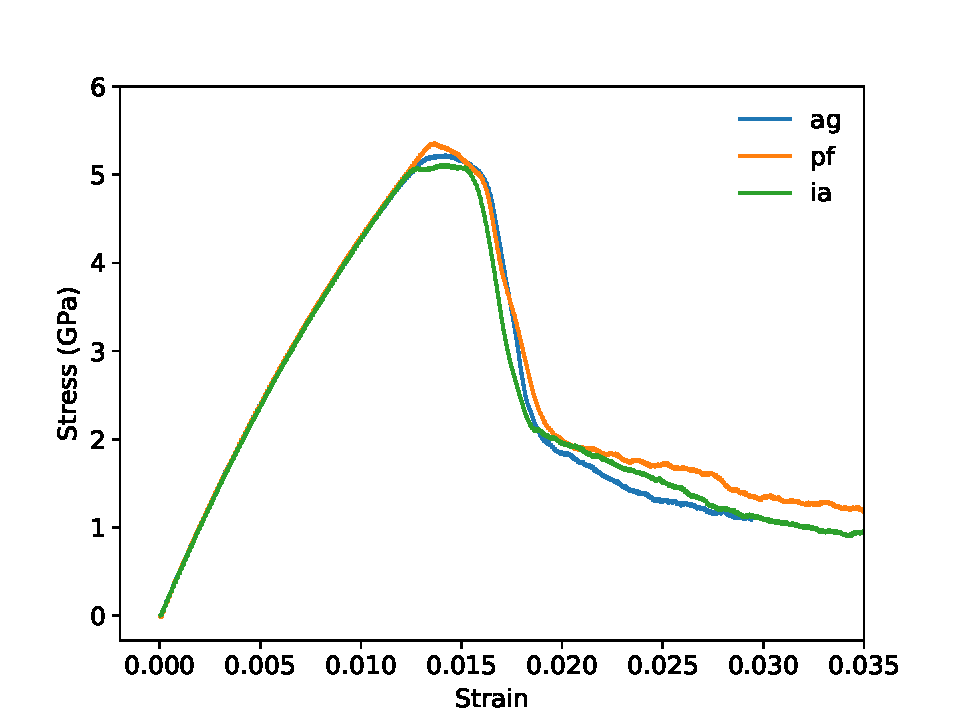
\includegraphics[width=1\linewidth]{img/allline}
		\centering
		\caption{Stress-strain response of models}
		\label{fig:stress&strain}
	\end{minipage}	
	\hfill
	\begin{minipage}{0.495\textwidth}		
		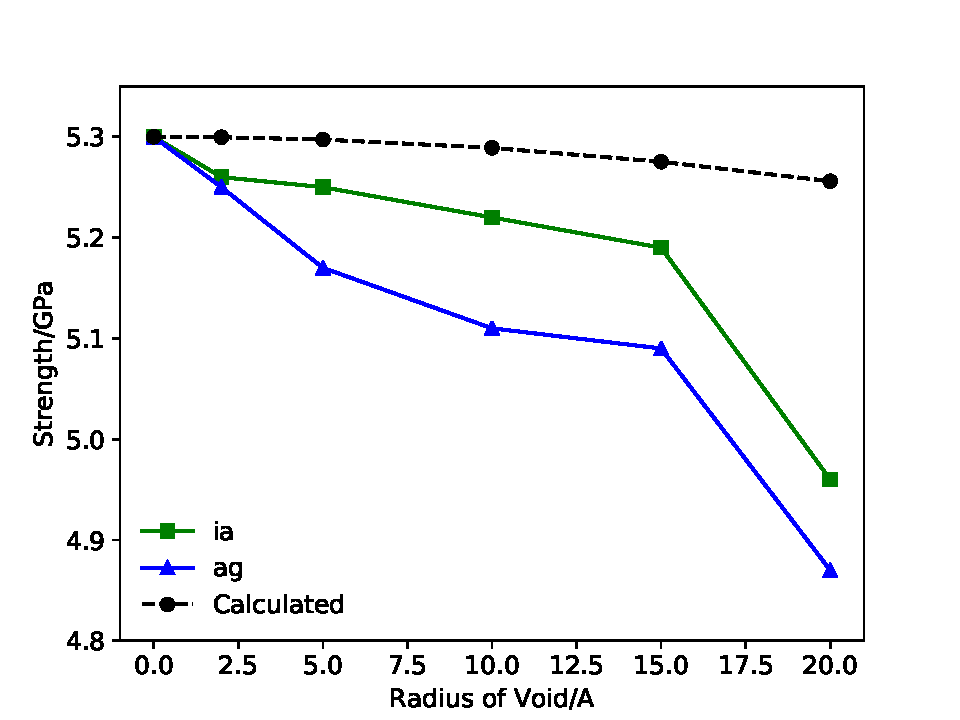
\includegraphics[width=1\linewidth]{img/effect_of_vol}
		\centering
		\caption{Yield strength of material with void}
		\label{fig:strength}
	\end{minipage}
\end{figure}


%%%	
%\begin{figure}[ht]
%%	\includegraphics[width=1\linewidth]{"img/fracture3"}
%	\caption{Yield process of the models}
%	\label{fig:yield}
%\end{figure}
	
It has been observed in Fig. \ref{fig:strength} that voids detract the strength of  materials. The max stress  of the simulation cell decreases as the volume of voids increases. It can be seen from Fig. \ref{fig:stress&strain}, there is a critical value of void radius about 15 \AA, the void greater than 15 \AA\ causes serious detraction of strength of material.  The decrease rate of loading area are smaller compared with the detraction of strength, so it can be assumed that the  yield behavior and strength is more related with local behavior of grain boundaries and void. Grain and phase boundaries are obstacles to deformation, thus the stability of boundaries have a great impact on the strength of materials. Interactive between grain boundary and void determines the fracture mode of   Ti-Al alloy.




\subsection{Evolution of spherical void}
The role of void can be concluded as two main parts: source of dislocations and obstacles to dislocations, which is dominant depends on the location of void. Void inside $\alpha_2$ phase plays a role of inclusion, in other words, this type of void possesses similar properties as second phase particles.
 
\begin{figure}[ht]
	\centering
	\includegraphics[width=1\linewidth]{"img/orowan"}
	\caption{Orowan process in $\alpha_2$-phase (atoms with regular arrangement have been removed)}
	\label{fig:orowan}
\end{figure}
Void inside $\alpha_2$ phase induced considerable misfit-stress fields and thus can influence material properties pronouncedly. Such stress fields surrounding the second-phase particles can be due to misfit between $\alpha_2$ phase atoms and surface atoms surrounding the void. That's a possibly favorable effect of second-phase particles that void contribution to the enhancement of mechanical strength. The strengthening effect of the particle inside single phase TiAl alloy has been verified by experiment \cite{Zghal1998}. Considering yielding of a material as related to glide of dislocations, any mechanism obstructing dislocation glide improves the mechanical strength. The defect evolution neighboring the void during yield stage is shown in Fig. \ref{fig:orowan}(a), the role of void is similar to second-phase particles. It functions as obstacles for dislocation migration which is shown by Fig. \ref{fig:orowan}(b): the stress fields surrounding the second-phase particles block migrating dislocation, the void particle acts as pinning point. The dislocation can pass two pinning points under shear  stress , and the critic value depends on the distance between  obstacles, it is be given by \cite{Xiong2015}:
\begin{equation} \label{eq:orowan} 
\tau_0 = Gb/d
\end{equation}
where $d$ represents the distance between two obstacles A and B in Fig. \ref{fig:orowan} , reflects the dependence of the critical shear stress $\tau_0$ on the second-phase particle density and distribution. This mechanism for hardening is designated as the Orowan process with $\tau_0$ as the Orowan shear stress. As a result of the Orowan process, upon passage of the pinning points by a series of gliding dislocations, a system of concentric loops is formed around the second-phase particles. Consequently, the effective average distance between the second phase particles has decreased to $d$ which implies a necessary increase of the value of critical shear stress required for continuation of dislocation glide. The width of a burgers vector, will be generated at both sides of a crystal along the direction of burgers vector after dislocation traversing the entire crystal, as is shown in the third subfigure of Fig. \ref{fig:orowan}(b). 

\begin{figure}[ht]
	\centering
	\includegraphics[width=1\linewidth]{"img/void-gb"}
	\caption{(a) Fracture mode of two types of model  (b)Evolution of void at  phase boundary}
	\label{fig:void-gb}
\end{figure}
Effect of voids at different positions on the crack mode of the material are shown by Fig. \ref{fig:void-gb}(a). The model with void fractured cross the grain, and the model with void at $\alpha_2 / \gamma$ boundary resulted a large crack along the boundary under tensile loading. The difference of crack mode can attribute to the position of void and the evolution of the defect. Nucleation, emission of Shockley partial dislocation affects the evolution of the void at boundary greatly due to the anisotropy of two phases on the both sides of the phase boundary. The void weakened the strength of the grain it locates, $\alpha_2$ phase grain is easy to deformed under shear stress, thus that caused the crack initiated inside grain and finally caused fracture across the grain. Deformation mechanism of the model with void at boundary is more complex due to the interaction between void and phase boundary. In elastic stage, the system composed of $\alpha_2$ phase, $\gamma$ phase and void is in equilibrium, internal stress are balanced under compatible deformation as is shown by the first subfigure of Fig. \ref{fig:void-gb}(b). In the middle moment of yield stage, partial dislocation with Burgers vector $1/6[\overline{2}\ \overline{1}\ 1]$ emitted from surface of void in Fig. \ref{fig:void-gb}(b)-2. The micro crack initialed from the zone neighboring the interface between void and boundary, that quickly caused abrupt decohension of phase boundary. That accounts for the reason that material with void at $\alpha_2 / \gamma$ phase boundary is weaker than other cases. 
\section{conclusion}
In this paper, deformation behavior of two phase Ti-Al alloy under tensile loading was simulated with MD method. The mechanism of deformation was investigated under atomic scale, and the effect of void on the properties of two phase Ti-Al alloy was also studied.  The conclusions are as follows:\\
(1) Major deformation component of the two phase TiAl alloy is $\gamma$ phase, $\alpha_2$ phase is harder to be deformed, this inhomogeneity results in cracks at interface of the two phases. \\
(2) Effect of  void on the strength of the two phase alloy is sensitive to the location of  void. Void inside grain has detraction to the strength of material because the strengthening mechanism similar to second phase particle. Void at $\alpha_2 / \gamma$ boundary is most risky situation for two phase alloy because of fast fracture along boundary.

\reftitle{References}
\bibliography{ref/VIOLET-ref.bib}
\funding{This research was funded by the National Natural Science Foundation of China (No. 51665030) and the Program for Changjiang Scholars and Innovative Research Team in Universities of the Ministry of Education of China (No. IRT-15R30), the Hongliu First-class  Disciplines Development Program of Lanzhou University of Technology, and the Doctoral Research Foundation of Lanzhou University of Technology.}

\end{document}



